\chapter{Proprietà topologiche}
Se esiste una categoria di proprietà che è fondamentale avere bene a mente in topologia, queste sono le proprietà topologiche. 
In sostanza diciamo \textbf{proprietà topologica} una caratteristica invariante per omeomorfismi; vedremo presto come applicarle allo studio della topologia generale che abbiamo appena completato.



\section{Proprietà di Hausdorff $T_2$}
 \subsection{\textcolor{TopGener}{\textbf{La proprietà $T_2$}}}
 
 
 
\begin{definition}
	Sia $(X, \tau)$ spazio topologico, è detto \textbf{di Hausdorff} (o $T_2$) se $\forall \ x, y, x \neq y$ esistono due intorni $U, V \in \mathcal{N}_\tau(x),\mathcal{N}_\tau(y)$ tali che $U \cap V = \varnothing$.
\end{definition} 


La proprietà di Hausdorff è detta $T_2$,  esistono anche $T_0, T_1, T_3, T_4$, altre proprietà più deboli o più forti (a seconda della loro numerazione) di quella di Hausdorff. \\ La più forte, $T_4$, richiede che in due insiemi chiusi disgiunti ogni intorno dei loro punti sia disgiunto e viene anche detta \textbf{normalità}. La più debole, $T_1$, richiede che i sottoinsiemi singoletti di $X$ siano chiusi.\\ \\ Esistono interessanti relazioni tra le varie proprietà $T_i$, ad esempio $T_2$ implica $T_1$ ma l'inverso non vale. \footnote{si veda un insieme $X$ infinito con topologia cofinita, è immediato verificare che vale come controesempio.}

\begin{remark}
	La condizione di Hausdorff è topologica. \\  Infatti è preservata dagli omeomorfismi: vale che
	\begin{center}
		$(X,\tau)$ è di Hausdorff se e solo se anche $(Y,\xi)$ è di Hausdorff ed esiste $\morphism{f}{(X,\tau)}{(Y,\xi)}$ omeomorfismo tra i due spazi topologici
	\end{center}
	 Se $x,y \in X$ e $x\neq y$, allora $f(x), f(y) \in Y$ e $f(x) \neq f(y)$ poiché $f$ biettiva. Se esistono degli $U,V\in \mathcal{N}_\tau(x),\mathcal{N}_\tau(y)$ tali che $U \cap V = \varnothing$, esistono $A \subset U$ e $A' \subset V$ aperti tali che $A \cap A' = \varnothing$. Per cui $f(A) \cap f(A') = \varnothing$, dove $f(A), f(A')$ sono aperti ed intorni rispettivamente di $f(x),f(y)$. Quindi la proprietà vale. Inoltre applicando l'inversa si ottiene l'altra implicazione.
\end{remark} 
\begin{remark}
	Se $(X, \tau)$ è di Hausdorff, allora ogni topologia più fine $\tau \subset \xi$ è di Hausdorff su $X$. \\ Infatti interessano soltanto gli aperti \textit{più piccolini} e non quelli grossi. Se ci sono aperti più piccoli e sappiamo che ce ne sono già di piccoli abbastanza affinché sia Hausdorff, non danno problema. Se ci sono aperti più grossi, non è interessante comunque, perché per la proprietà di Hausdorff ci servono \textit{aperti abbastanza piccoli}. \\ Se si volesse proprio fare una dimostrazione: sia $x \neq y$ allora $\tau \subset \xi$ per cui esistono in $\tau$ $U \cap V = \varnothing$ e quindi $U, V$ sono ancora intorni in $\xi$, pertanto anche $\xi$ è di Hausdorff. 
\end{remark}
\begin{remark}
	Sia $(X, \tau)$ spazio topologico, se per ogni $A, B\in \tau$ si ha che $A\cap B \neq \varnothing$ allora $\tau$ non è di Hausdorff. \\ Infatti per ogni coppia di intorni $U, V$ di $x, y$ (rispettivamente) si ha che esistono $A \subset U, A' \subset V$ tali che $\varnothing \neq A\cap A' \subset U \cap V$
\end{remark} 

\begin{example} \
\begin{enumerate}
	\item Le topologie metrizzabili sono di Hausdorff, in particolare la topologia discreta lo è. 
	\item La topologia banale su un insieme $X$ di cardinalità maggiore di $2$ non è di Hausdorff. 
	\item La topologia cofinita su un insieme infinito non è di Hausdorff. Per osservazione precedente, basta dimostrare che ogni aperto ha intersezione non vuota. Per cui siano 
	\begin{equation*}
	A \cap B = F^c \cap G^c = (F \cap G)^c 
	\end{equation*}
	ma $F\cap G$ è finito quindi il complementare è non vuoto. 
\end{enumerate}
\end{example}

\begin{theorem}
	Sia $(X, \tau)$ spazio topologico e sia $\varnothing \neq S \subset X$, allora se $(X, \tau)$ è di Hausdorff $(S, \tau|_S)$ è di Hausdorff. 
\end{theorem} 
\begin{proof}
	Fisso $x,y \in S \subset X$ qualsiasi, purché $x \neq y$. Allora prendendo un intorno per ciascun punto tale da soddisfare la condizione di Hausdorff; ho che $U \cap V = \varnothing$. Ma $U \cap S = U' \in \tau|_S$ e $V \cap S = V' \in \tau|_S$ e dunque se $U \cap V = \varnothing \Longrightarrow U \cap V \cap S = U' \cap V' = \varnothing$. Ovvero anche la topologia $\tau|_S$ è di Hausdorff.
\end{proof}

\begin{theorem}
	Siano $(X_1, \tau_1)$ e $(X_2, \tau_2)$ spazio topologico e $(X_1 \times X_2, \tau)$ la topologia prodotto delle prime due. \\Allora $(X_1 \times X_2, \tau)$ è di Hausdorff se e solo se $(X_1, \tau_1)$ e $(X_2, \tau_2)$.
\end{theorem} 
\begin{proof} \
	\begin{enumerate}
		\item Si fissino $(x_1, y_1), (x_2, y_2) \in X_1 \times X_2$. Allora $\left\{x_1\right\} \times X_2 \simeq X_2$ e sappiamo che è di Hausdorff per ipotesi, analogamente per $X_1 \times \left\{y_1\right\} \simeq X_1$ e quindi è di Hausdorff. Pertanto posso trovare un intorno $U \times \left\{y_1\right\} \cap U' \times \left\{y_1\right\} = \varnothing$ con $x_1 \in U$ e $x_2 \in U'$; analogamente $\left\{x_1\right\} \times V \cap \left\{x_1\right\} \times V' = \varnothing$ con $y_1 \in V$ e $y_2 \in V'$. Per la definizione di intorni ho degli aperti tali che 
		\begin{equation*}
		A \times B \cap A' \times B' \subset (U \times V) \cap (U' \times V') = (U \cap U') \times (V \cap V') = \varnothing
		\end{equation*}
		Ma $A \times B$ e $A' \times B'$ sono aperti di $\tau$ e dunque sono anche intorni dei due punti. Quindi ho trovato due intorni la cui intersezione è vuota. $X_1 \times X_2$ è di Hausdorff.
		\item Fisso $\left\{x_1\right\} \subset X_1$, $\left\{x_2\right\} \subset X_2$ e considero $X_1 \times \left\{x_2\right\}$ e $\left\{x_1\right\} \times X_2$,per la proposizione precedente sono di Hausdorff e sono omeomorfi rispettivamente a $X_1$ e $X_2$. Pertanto $X_1$ e $X_2$ sono di Hausdorff.
	\end{enumerate}
\end{proof}

\begin{remark}
Se uno degli $X_1$ è di Hausdorff ed $X_2$ non è di Hausdorff, allora il loro prodotto non è di Hausdorff. \\ Per esempio si consideri il prodotto tra $\R$ con la topologia euclidea e la topologia banale su $\R$. Allora il prodotto non è di Hausdorff perché $(1,1)$ e $(1,2)$ sono distinti ma stanno sempre nello stesso intorno. 
	
	% TODO: se valesse $X_1$ $T_2$ e $X_2$ $T_1$ il prodotto sarebbe di Hausdorff?
\end{remark} 


\begin{remark}
	In generale il passaggio a quoziente non è di Hausdorff anche se l'insieme di partenza è di Hausdorff. \\ Infatti si consideri il diagramma 
	\begin{equation*}
	\begin{tikzcd}[row sep = 3em]
	 (X, \tau_{\text{euclidea}}) \arrow{d}{\pi}\arrow{r}{f} & (Y, \tau_f)\\
	(X/R,\tau_{X/R}) \arrow[swap]{ru}{\simeq} &
	\end{tikzcd}
	\end{equation*}
	dove $f = \mathcal{X}_{\left[0,2\right)}$. La funzione induce (per quanto visto precedentemente) la topologia banale e quindi non di Hausdorff malgrado la topologia euclidea sia Hausdorff. 
\end{remark} 



\subsection{\textcolor{TopGener}{\textbf{La proprietà $T_1$}}}



\begin{definition}
	Sia $(X, \tau)$ spazio topologico, allora si dice \textbf{$T_1$} se i suoi singoletti sono chiusi. 
\end{definition}

\begin{theorem}
	Se vale che $(X, \tau)$ soddisfa $T_2$ ovvero è di Hausdorff, allora è anche $T_1$.
\end{theorem} 
\begin{proof}
	Devo dimostrare che per ogni $x\in X$, $\left\{x\right\}$ è un chiuso. Quindi mi basta dimostrare che $\left\{x\right\}^c$ è aperto. Per cui sia $y \in \left\{x\right\}^c$, per la proprietà di Hausdorff dev'essere che esiste $U \in \mathcal{N}_\tau(y)$ ho che $U \cap V = \varnothing$ dove $V$ è un intorno di $\left\{x\right\}$. Per cui dev'essere che $U \subset \left\{x\right\}^c$ per qualche $U$ intorno. Ovvero $\left\{x\right\}^c$ è intorno di tutti i suoi punti e quindi è un aperto e $\left\{x\right\}$ è un chiuso.
\end{proof}

\begin{theorem}
	Sia $\left\{x_n\right\}$ una successione definita su $(X, \tau)$ spazio topologico di Hausdorff allora se converge allora converge ad un solo punto. 
\end{theorem} 
\begin{proof}
	È sempre la solita dimostrazione che in $\R$ se il limite converge allora non può avere due valori distinti. Ma comunque la ripresento anche qui. Suppongo che una successione $\left\{x_n\right\}_{n \in \N} \rightarrow \left\{k_1, k_2\right\}$, allora per definizione di convergenza in uno spazio topologico ho che per ogni intorno di $k_1$ c'è sempre almeno un punto della successione. Per cui prendo un intorno $U$ di $k_1$ e uno $V$ di $k_2$ tale che $U \cap V = \varnothing$ che esistono per la proprietà di Hausdorff. Se la successione converge in entrambi i punti allora $U \cap V \neq \varnothing$. Da questo assurdo si arriva a concludere che una successione, se converge, converge ad un solo punto in uno spazio di Hausdorff. 
\end{proof}

\begin{theorem}
	Sia $\left\{x_n\right\}_{n\in \N}$ una successione in $(X,\tau)$ spazio topologico di Hausdorff che soddisfa il primo assioma di numerabilità, allora se $x \in X$ è un punto di accumulazione di $\left\{x_n\right\}_{n\in \N}$ esiste una sottosuccessione tale che $\left\{x_{n_k}\right\}_{n_k \in \left\{n_k\right\}_{k \in \N}} \rightarrow x$. 
\end{theorem}

\begin{remark}
	Sia $(X, \tau)$ spazio topologico che soddisfa $T_1$, allora non vale che una successione converga ad un unico punto.
\end{remark}

\begin{theorem}
	\begin{equation*}
	(X, \tau) \; \text{è} \; T_2 \Leftrightarrow \Delta_{X} \; \text{è chiuso} \; X \times X
	\end{equation*}
\end{theorem} 
\begin{proof} \
	Bisogna innanzitutto far notare che $U \cap V = \varnothing \Leftrightarrow \Delta_X \cap (U \times V) = \varnothing$.
	\begin{enumerate}
		\item[$(\Rightarrow)$] Poiché $T_2$ posso prendere $U, V \in \mathcal{N}_\tau(x)$ tali che $U \cap V = \varnothing$, allora $\Delta_X \cap (U \times V) = \varnothing$; $\Delta_X$ è aperto in $X\times X$ e $\Delta_X$ è chiusa. 
		\item[$(\Leftarrow)$] Se $\Delta_X$ chiuso $\Delta^c_X$ è aperto, quindi posso pendere un intorno di un punto interno di $\Delta^c_X$ tale che $U \cap \Delta_X = \varnothing$. Inoltre ogni intorno $U = U' \times V'$ dove $U', V'$ è in $X$, perciò $(U' \times V') \cap \Delta_X = \varnothing$. Per l'osservazione iniziale $U' \cap V' = \varnothing$.
	\end{enumerate}
\end{proof}

\begin{theorem}
	Siano $\morphism{f,g}{(X,\tau)}{(Y,\xi)}$ continue, $Y$ è $T_2$ se e solo se $Z \coloneqq \left\{x \in X \,\middle|\, f(x) = g(x) \right\}$ è chiuso in $X$.
\end{theorem}
\begin{proof}
	% TODO
\end{proof}



\section{Compattezza}
\subsection{\textcolor{TopGener}{\textbf{Spazi e sottospazi compatti}}}



\begin{definition}
	Sia $(X, \tau)$ spazio topologico, si dice \textbf{compatto} se da ogni ricoprimento aperto di $X$ è possibile estrarre un sottoricoprimento aperto finito di $X$. \\ \\ Ovvero sia $\left\{A_i\right\}_{i\in I}$ una famiglia di insiemi aperti tali che
	\begin{itemize}
		\item $A_i \in \tau \ \forall \ i\in I$
		\item $\bigcup_{i \in I} A_i = X$
	\end{itemize}
	allora posso estrarre un $J \subset I$ con $|J| < +\infty$ e $\bigcup_{i \in J} A_i = X$
\end{definition} 

\begin{example} Spazi topologici compatti:
\begin{enumerate}
	\item Ogni spazio con la topologia banale.
	\item $X$ finito con qualsiasi topologia è finito.
	\item $(X, \tau_{cof})$ con $|X| \ge +\infty$ è compatto. Infatti da un qualsiasi ricoprimento si prenda uno degli aperti $A_{i_0}$, allora $X \setminus A_{i_0} = \left\{x_1, \dots, x_n\right\}$ per qualche $n < +\infty$. Pertanto bastano al più $n+1$ insiemi per ricoprire l'insieme.
	\item $(X,\tau_{\text{discreta}})$ dove $|X| \ge +\infty$  non è compatto perché basta prendere il ricoprimento dei singoletti.
	\item $(\R, \tau_{\text{euclidea}})$ non è compatto. Infatti basta prendere la famiglia $\left\{(-n, n)\right\}_{n \in \N_{>0}}$ per vedere che non è compatto. Se si estraggono un numero finito di elementi da quella famiglia e si prendono gli indici in $J$ tale che $|J| = d < +\infty$ allora $\bigcup_{j \in J}(-n_j, n_j) = (-\max_{j \in J} n_j,  \max_{j \in J} n_j)$ che non ricopre tutto $\R$.
\end{enumerate}
\end{example}

\begin{definition}
	Sia $(X, \tau)$ spazio topologico e $S \in 2^X$ si dice che $S$ è un \textbf{sottospazio compatto} in $(X, \tau)$ se lo è il corrispondente spazio $(S, \tau|_S)$.
\end{definition} 

\begin{remark}
	$S$ è compatto se e solo se ogni volta che prendo un ricoprimento $\left\{A_i\right\}_{i \in I}$ in $\tau$ di $S$ riesco a estrarre un sottoricoprimento finito tale che $\bigcup_{i \in J} A_i \supset S$ 
	\begin{proof}
		$S$ è compatto se e solo se posso trovare un ricoprimento $\left\{A_i\right\}_{i \in I}$ da cui estraggo un sotto ricoprimento finito $\left\{A_i\right\}_{i \in J}$, ma ciascuno di quegli $A_i = A'_i \cap S$ per qualche $A'_i \in \tau$. Per cui ho che è anche un ricoprimento finito di $S$ in $\tau$, infatti sia $\left\{A'_i\right\}_{i\in J}$, vale 
		\begin{equation*}
			S = \bigcup_{i \in J} A_i = \bigcup_{i \in J} (A'_i \cap S)  \subset  \bigcup_{i \in J} A'_i
		\end{equation*}
		analogamente nell'altro verso si vede che si può prendere il ricoprimento aperto estrarre le parti significative e ottenere un nuovo ricoprimento nella sottotopologia.
	\end{proof}
\end{remark}



\subsection{\textcolor{TopGener}{\textbf{Caratteristiche degli spazi compatti}}}



\begin{theorem}[Heine-Borel]
	Ogni intervallo chiuso e limitato in $\left[a, b\right]$ per ogni $a, b$ tale che $a < b$ di $\R$ con $\tau_{\text{euclidea}}$.
\end{theorem} 
\begin{proof}
	Dato un ricoprimento $\left\{A_i\right\}_{i \in I}$ 
	\begin{equation*}
			Y \coloneqq \left\{ x\in \left[a,b\right] \,\middle|\, \exists J \subset I. \; \text{t. c.} \; |J| < +\infty,\ \bigcup_{j \in J} A_j \supset \left[a,x\right] \right\}
	\end{equation*}
	È ovvio che $a \in Y$, per cui $Y \neq \varnothing$ ed essendo $Y \subset \R$ allora esiste $\sup Y =: z$. \\ Poiché $z \in \left[a,b\right]$ e l'intervallo è ricoperto dagli $A_i$, deve esistere un $A_{k}$ tale che $z \in (z-\varepsilon, z+\varepsilon) \subset A_k$ per qualche $\varepsilon > 0$, visto che $A_i$ aperto. Inoltre per la definizione di estremo superiore so che per qualsiasi $\varepsilon$ esiste un $x$ tale che $x \in \left[z-\varepsilon, z\right] \cap Y$. Quindi posso costruire il seguente ricoprimento:
	\begin{align*}
		\left[a,z+\varepsilon\right] & = \left[a,x\right] \cup \left[z-\varepsilon, z+\varepsilon\right]\\
				& =  \bigcup_{j \in J' \subset I} A_i \cup A_k
	\end{align*}
	dove $J'$ è un sottoinsieme finito. Segue ovviamente che $z = b$, infatti se non lo fosse allora non potrebbe essere l'estremo superiore di $Y$ visto che $z+\varepsilon > z$, ed è ottenuto attraverso un ricoprimento finito. Inoltre il ricoprimento ottenuto contiene $z = b$. $\left[a,b\right]$ è compatto.
\end{proof}

\begin{remark}
	Esistono spazi topologici compatti che possiedono sottoinsiemi non compatti. Per esempio si prenda $(\left[a, b\right],\tau_text{euclidea})$; il sottoinsieme $(0, 1)$ è un insieme non compatto. 
\end{remark} 

\begin{theorem} \
	\begin{enumerate}
		\item Un sottoinsieme $S$ chiuso in $(X, \tau)$ spazio topologico compatto $S$ è compatto. 
		\item Un sottoinsieme compatto $S$ in uno spazio topologico di Hausdorff $(X,\tau)$ è chiuso. 
	\end{enumerate}
\end{theorem} 
\begin{proof} \
	\begin{enumerate}
		\item Si noti che se $S$ è chiuso allora $S^c$ è aperto. Quindi prendo un ricoprimento di $S$ aperto in $\tau|_S$ che denoto con $\left\{A_i\right\}_{i \in I}$ se aggiungo a questo ricoprimento $S^c$ allora considero $\left\{A'_i \cup S^c\right\}_{i \in I}$ dove $A_i = A'_i \cap S$ e $A'_i \in \tau$. Per cui questo è un ricoprimento aperto di $(X,\tau)$. Per la compattezza posso estrarre un sottoricoprimento finito tale da ricoprire tutto $X$ che sarà costituito da elementi $\left\{A'_j \cup S^c\right\}_{j \in J}$ dove $|J| < +\infty$. Ovviamente vale
		\begin{equation*}
			S \subset \bigcup_{j \in J} A'_j \cup S^c \Longrightarrow S = S \cap S \subset \bigcup_{j \in J} (A'_j \cup S^c) \cap S = \bigcup_{j \in J} A'_j  \cap S
		\end{equation*}
		dove gli $A'_j \cap S \in \tau|_S$ e quindi ho trovato un sottoricoprimento finito aperto di $S$.  
		\item 
		% TODO riscrivere se ho vena artistica
		Voglio far vedere che ogni $p \in S^c$ ha come intorno $S^c$ e dunque affermare che $S$ è chiuso in $\tau$. Per cui fissato un $p \in S^c$, per ogni $x \in S$ esistono due intorni $U_x, V_x \in \mathcal{N}_\tau(x), \mathcal{N}_\tau(p)$ tali che $U_x \cap V_x = \varnothing$ (poiché $X$ è di Hausdorff). Per cui dato un $U_x$ posso scegliere $x \in A_x \subset U_x$ per definizione di intorno e, tale che $A_x \cap V_x = \varnothing$. Prendendo tutti questi $A_x$, una volta fissato un $p \in S^c$, si può ottenere un ricoprimento aperto di $S$, rappresentato dalla famiglia $\left\{A_x\right\}_{x \in S}$. \\ Essendo $S$ compatto posso estrarre un sottoricoprimento aperto finito  $\left\{A_{x_j}\right\}_{j \in J}$ dove $|J| < +\infty$, così da ottenere rispettivamente una famiglia di intorni di $p$ finita (infatti per le osservazioni precedenti per ogni $U_x$ esisteva un $V_x$). Prendendo il minimo tra questi intorni, ovvero la loro intersezione finita che denoto con $V$, si ottiene ancora un intorno con $p \in V \subset S^c$. Poiché vale per ogni $p \in S^c$ ho dimostrato che $S^c$ è intorno di ogni suo punto e quindi $S^c \in \tau$. 
	\end{enumerate}
\end{proof}

\begin{remark}
	Se siamo in uno spazio topologico compatto ma non $T_2$, per esempio $(\R, \tau_{cof})$, allora un suo sottoinsieme compatto non è anche chiuso. \\ Infatti se si prende $\left[0,1\right] \subset \R$ nella topologia cofinita questo è compatto, ma non è chiuso (se fosse chiuso allora $\#\left[0,1\right] < +\infty$, che è falso)
\end{remark}

\begin{corollary}
	Sia $\varnothing \neq S \subset \R$ in $(\R, \tau_{\text{euclidea}})$. \\ $S$ è compatto se e solo se è chiuso e limitato. 
\end{corollary} 
\begin{proof}
	\begin{enumerate}
		\item[$(\Rightarrow)$] Poiché $S$ compatto allora è chiuso perché siamo in $\R$ che è $T_2$. Inoltre supponiamo $S$ illimitato, allora vale $(-n, n) \cap S \neq S$ per qualsiasi $n \in N$. Quindi posso prendere il ricoprimento $\left\{(-n,n)\right\}_{n\in \N}$ che ricopre tutto $\R$, ma per quanto osservato precedentemente non esiste un ricoprimento finito tale da ricoprire $S$.
		\item[$(\Leftarrow)$] Essendo limitato deve esistere $S\subset \left[a,b\right]$. Quindi $\left[a,b\right] \cap S$ è chiuso perché intersezione di chiusi. Ma $\left[a,b\right]$ è un compatto per Heine-Borel, e per il lemma precedente un chiuso in un compatto è ancora un compatto, ovvero $S$ dev'essere compatto.
	\end{enumerate}	
\end{proof}

\begin{theorem}[L'immagine di un compatto è compatta]
	Siano $(X, \tau)$ spazio topologico compatto, $(Y, \xi)$ spazio topologico, $\morphism{f}{X}{Y}$ continua. \\ Allora $f(X)$ è un sottoinsieme compatto. 
\end{theorem} 
\begin{proof}
	Si consideri un ricoprimento aperto di $f(X)$ indicato con $\left\{A_i\right\}_{i \in I}$. Allora visto che i suoi elementi sono tutti aperti segue che $f^{-1}(A_i) \in \tau$. \\ Poiché $f(X)$ è l'immagine di $X$ attraverso $f$, dev'essere che la controimmagine del ricoprimento sia proprio $X$. Ma $X$ è un compatto, quindi dato un suo ricoprimento aperto, in questo caso sarà $\left\{f^{-1}(A_i)\right\}_{i \in I}$, posso estrarne uno finito che dico $\left\{f^{-1}(A_j)\right\}_{j \in J}$ dove $J \subset I$ e $|J| < +\infty$. Rimandando in avanti le controimmagini (ricordando che l'immagine commuta con l'unione!) risulta che
	\begin{equation*}
		X = \bigcup_{j \in J} f^{-1}(A_j) \Longrightarrow f(X) = \bigcup_{j \in J} f(f^{-1}(A_j)) \subset \bigcup_{j \in J} A_j
	\end{equation*}
	e quindi ho trovato un sottoricoprimento aperto e finito di $f(X)$.
\end{proof}

\begin{corollary}[Weierstrass]
	Sia $(X, \tau)$ uno spazio topologico compatto e sia $\morphism{f}{X}{\overline{\R}}$ continua, allora $f(X)$ ammette massimo e minimo in $X$.
\end{corollary} 
\begin{proof}
	$f(X)$ compatto, quindi $f(X)$ è un insieme chiuso e limitato per cui deve contenere massimo e minimo.
\end{proof}

\begin{theorem}[Tychonoff]
	Lo spazio topologico $X_1 \times X_2$ è compatto se e solo se $X_1,X_2$ sono compatti. 
\end{theorem} 
\begin{proof}
	\begin{enumerate}
		\item[$(\Rightarrow)$] Se $X_1 \times X_2$ è compatto e $\pi_1, \pi_2$ sono le proiezioni canoniche, allora per la continuità segue che $\pi_i(X_1 \times X_2)$ dev'essere compatto e per la surgettività $ \pi_i(X_1 \times X_2) = X_i$; segue che $X_i$ è compatto per $i \in \left\{1,2\right\}$.
		\item[$(\Leftarrow)$] Sia $\left\{U_j\right\}_{j \in J}$ un ricoprimento di $X_1 \times X_2$, allora vale che $U_j = \bigcup_{h \in H_j} V_h \times W_h$ (dove $V_h \in \tau_1$ e $W_h \in \tau_2$). \\ Sapendo che $\left\{x\right\} \times X_2 \simeq X_2$ per ogni  $x \in X_1$, dev'essere che anche $\left\{x\right\} \times X_2$ è compatto. In particolare ho che 
		\begin{equation}
		\begin{aligned}
			\left\{x\right\} \times \subset \bigcup_{h \in h(x)} V_h \times W_h
		\end{aligned}
		\end{equation}
		dove $h(x) \subset H$, per cui vale la relazione sopra ed $h(x)$ è ovviamente finito (posso verificarlo per la compattezza di $X_2$). Si può osservare che per ogni $h \in h(x)$ deve valere $x \in V_h$, e quindi definisco per ogni $x \in X_1$ il seguente ricoprimento aperto 
		\begin{equation*}
			V(x) = \bigcap_{h \in h(x)} V_h
		\end{equation*}
		con $V(x) \in \tau_1$ poiché intersezione finita di aperti. Inoltre essendo che 
		\begin{equation*}
			\bigcup_{x \in X_1} V(x) = X_1
		\end{equation*}
		posso estrarre un sottoricoprimento di $V(x)$ finito. A maggior ragione allora dev'essere che 
		\begin{equation*}
			\bigcup_{x \in X_1} \bigcup_{h \in h(x)} V_h = X_1
		\end{equation*} 
		quindi posso prendere $\left\{V_x\right\}_{x \in X_1}$ come ricoprimento e ottenere un sottoricoprimento finito aperto $V(x_1), \dots, V(x_n)$ di $X_1$. \\
		Per costruzione quindi posso estrarre un sottoricoprimento aperto finito  
		\begin{equation*}
			\bigcup_{x \in \left\{1,\dots, n\right\}} \bigcup_{h \in h(x)} V(x) \times W_h
		\end{equation*}
	\end{enumerate}
\end{proof}

\begin{corollary}
	Un sottoinsieme di $S \subset \R^n$ è compatto se e solo se è chiuso e limitato. 
\end{corollary} 
\begin{proof}
	% TODO
\end{proof}

\begin{theorem}
	$\morphism{f}{X}{Y}$ continua con $(X, \tau)$ compatto e $(Y, \xi)$ di Hausdorff. Allora $f$ è chiusa. \\ In particolare se $f$ è biettiva allora è un omeomorfismo. 
\end{theorem} 
\begin{proof}
	Se fisso $C$ chiuso in $(X,\tau)$ allora $C$ è compatto, quindi $f|_C(C)$ è un compatto e siccome il codominio è di Hausdorff dev'essere che $f|_C(C)$ è anche chiuso. La seconda parte è banale per caratterizzazioni precedenti.
\end{proof}

\begin{corollary}
	\label{thr:freeomeombyquo}
	Sia $(X, \tau)$ spazio topologico compatto, $(X', \tau')$ di Hausdorff e $R$ relazione su $X$. Se esiste $\morphism{f}{(X, \tau)}{(X', \tau')}$ e $f$ continua e surgettiva allora esiste una $g$ omeomorfismo tra $(X/R,\tau_{X/R})$ e $(X', \tau')$
\end{corollary}
\begin{proof}
	È ovvio, ma volevo sembrare saccente, quindi ecco una dimostrazione.
	Riprendendo il diagramma commutativo 
	\begin{equation*}
		\begin{tikzcd}[row sep = 3em]
			(X, \tau) \arrow[swap]{d}{\pi} \arrow{r}{f} & (X', \tau') \\
			(X/R_f, \tau_{X/R_f}) \arrow[swap]{ru}{\exists! g} &
		\end{tikzcd}	
	\end{equation*}
	sappiamo che esiste $g$ biettiva. Ma dalle condizioni sopra sappiamo anche che $(X,\tau)$ è compatto e poiché $\pi$ è continua anche $X/R_f$ è compatto. Per cui $g$è da un compatto ad uno spazio di Hausdorff, e applicando il teorema sopra a $g$ otteniamo un omeomorfismo. 
\end{proof}



\section{Connessione}
\subsection{\textcolor{TopGener}{\textbf{Spazi topologici connessi}}}



\begin{definition}
	Sia $(X, \tau)$ spazio topologico, si dice \textbf{connesso} se gli unici aperti e chiusi in $\tau$ sono $\varnothing, X$. \\ Si dice che $(X, \tau)$ è sconnesso se non è connesso. 
\end{definition} 

\begin{definition}
	Sia $S \subset X$, diciamo che \textbf{$S$ è connesso in $(X, \tau)$} se $(S, \tau|_S)$ lo è. 
\end{definition} 

\begin{theorem}
	Dato $(X, \tau)$ spazio topologico, le seguenti affermazioni sono equivalenti. 
	\begin{enumerate}
		\item $(X, \tau)$ è sconnesso. 
		\item $\exists A, B \in \tau$ tale che $A \cup B = X$ e $A \cap B = \varnothing$.
		\item $\exists A, B$ chiusi tali che $A\cap B = \varnothing$ e $A \cup B = X$.
	\end{enumerate}
\end{theorem} 
\begin{proof}
	È facile vedere che la condizione $1$ implica sia $2,3$ visto che esiste un insieme sia aperto che chiuso. Analogamente per le dimostrazioni $2,3 \Rightarrow 1$ che sono praticamente uguali, basta cambiare la parola aperto con chiuso. 
	\begin{enumerate}
		\item[$(1\Rightarrow 2,3)$] Se vale che è sconnesso allora esiste $A$ aperto e chiuso, allora posso prendere $A^c$ che è ancora aperto; quindi $A\cup A^c = X$, analogamente per $A$ chiusa. 
		\item[$(2 \Rightarrow 1)$] Si prende $A \cup B = X$, allora $B = A^c$ con $B$ ancora aperto, quindi esiste $A$ aperto e chiuso. 
	\end{enumerate}
\end{proof}

\begin{example}
\begin{enumerate}
	\item $(X, \tau_{\text{discreta}})$ con $|X| \ge 2$ allora ogni suo sottoinsieme è sconnesso. 
	\item $(X, \tau_{\text{banale}})$ è sempre connesso. 
	\item $(\R, \tau_{\text{euclidea}})$ sia $x \in \R$ è sconnesso infatti $\R \setminus \left\{x\right\}$ si può comporre con $(-\infty, x) \cup (x, +\infty)$ che sono sottoinsiemi disgiunti aperti e non vuoti. 
	\item Sia $|X| > + \infty$ allora $(X, \tau_{\text{cof}})$ è connesso basta vedere che i chiusi sono tutti finiti quindi non si può ricoprire $X$ con insiemi chiusi disgiunti. 
\end{enumerate}
\end{example}

\begin{definition}
	Sia $S \subset \R$, di dice \textbf{convesso} se per ogni $a, b\in S$ tali che $a \le b$ vale che se esiste $c\in \R$ tale che $a\le c\le b$ allora $c\in S$.
\end{definition} 

\begin{theorem}
	I connessi di $\R$ sono tutti e soli gli insiemi convessi. 
\end{theorem}
\begin{proof}
	Sia $J \subset \R$ convesso e supponiamo che sia sconnesso. Allora esistono $A, B$ chiusi in $\tau$, disgiunti e non banali, tali che $A \cap J \cup B \cap J = J$. Possiamo scegliere $a \in A \cap J$ e $b \in B \cap J$ con $a < b$ e per la convessità di $J$ deve essere che $\left[a,b\right] \subset J \subset A \cup B$. Considero $\sup \left[a,b\right] \cap A = x_0$ che esiste perché l'intersezione è non vuota. Inoltre $x_0 \in A$ poiché $A$ insieme chiuso. Quindi $x_0 \notin B$ e anche $x_0 \neq b$. Ma 
	\begin{equation*}
		\left(x_0, b\right] \subset \left[a,b\right] \setminus A \subset J \setminus A =  J \setminus (A \cap J) = B
	\end{equation*}
	chiudendo $\overline{\left(x_0, b\right]} = \left[x_0, b\right] \subset \overline{B} = B$ poiché $B$ è chiuso. Pertanto dev'essere che anche $x_0 \in B$. Allora non è vero che $A$, $B$ disgiunti visto che $x_0 \in A \cap B$. Da questo assurdo si dervia che $J$ è per forza connesso.\\
	
	Sia $S$ connesso, allora è anche convesso in $\R$. Se $S$ non fosse convesso: esistono $a,b,c \in \R$ tali che $a < c < b$ con $a,b \in S$ e $c \notin S$. Allora basta prendere $((-\infty, c) \cap S), ((c, +\infty) \cap S)$ come ricoprimento aperto disgiunto e quindi $S$ sarebbe sconnesso, che è un assurdo.
\end{proof}

\begin{remark}
	La connessione è una proprietà topologica. Infatti se $X \simeq Y$ e $X$ è connesso se è solo $Y$ è connesso. 
\end{remark} 

\begin{theorem}
	\label{thr:3.21.3}
	Siano $\morphism{f}{X}{Y}$ applicazione continua tra spazi topologici e $C$ insieme connesso di $X$, allora $f(C)$ è connesso. 
\end{theorem} 
\begin{proof}
	Se si restringe $f$ a $\morphism{f|_C}{C}{f(C)}$ questa è ancora continua, ma è anche suriettiva e $C$ è connesso. Pertanto possiamo lavorare con le ulteriori condizioni che il dominio sia connesso e $f$ suriettiva. Supponiamo che $f(C)$ sconnesso allora esistono due aperti $A, B \subset C$ disgiunti e non vuoti tali da ricoprire $f(C)$. Prendendo le controimmagini (ancora aperte perché continue), allora 
	\begin{equation*}
		f^{-1}(A) \cup f^{-1}(B) = f^{-1}(A \cup B) = f^{-1}(C) = C
	\end{equation*}
	ma $f^{-1}(A), f^{-1}(B) \neq \varnothing$ perché $f$ suriettiva, le fibre non si toccano perché è una funzione e quindi $f^{-1}(A) \cap f^{-1}(B) = \varnothing$. Per cui $C$ dev'essere sconnesso contro la nostra ipotesi Dev'essere quindi che anche $f(C)$ sia connesso.
\end{proof}

\begin{remark}
	Sia $X$ spazio topologico con $R$ relazione di equivalenza, $X/R$ è connesso se $X$ è connesso poiché $\morphism{\pi}{X}{X/R}$
\end{remark} 

\begin{definition}
	Sia $(X, \tau)$ spazio topologico e siano $x, y \in X$, si dicono \textbf{connessi $x, y$ in $(X, \tau)$} se esiste $S \subset X$ tale che è connesso e $x, y\in S$.
\end{definition} 

\begin{lemma}
	La relazione di connessione in $(X, \tau)$ è una relazione di equivalenza. 
\end{lemma} 
\begin{proof}
	Bisogna dimostrare che è riflessiva, simmetrica e transitiva.
	\begin{enumerate}
		\item	L'insieme $\left\{x\right\}$ è sempre connesso quindi $x$ è connesso con se stesso.
		\item L'insieme che connette $x,y$ connette anche $y,x$ visto che agli insiemi non "importa" l'ordine.
		\item La transitività è l'unica che richiede uno sforzo. Infatti siano $x,y$ connessi attraverso $A$ e $y,z$ connessi attraverso l'insieme $B$; se mostriamo che $A \cup B$ è connesso, $x$ è connesso con $z$. \\ Per cui sia $Y \subset A \cup B$ aperto e chiuso tale che $Y \neq \varnothing$. Per cui dev'essere che $Y \cap A \neq \varnothing$ o $Y \cap B \neq \varnothing$. Sia soltanto $Y \cap A \neq \varnothing$. Allora $Y \cap A$ è ancora aperto e chiuso poiché $Y$ aperto e chiuso nella topologia superiore. Ma $A$ è connesso, quindi dev'essere che $Y \cap A = A$ e dunque $A \subset Y$. Inoltre visto che $y\in A \cap B$, l'intersezione è non vuota e dev'essere che anche $Y \cap B \neq \varnothing$. Applicando un ragionamento analogo a quanto visto per $A$, segue che $B \subset Y$. Per cui $Y = A \cup B$, ovvero gli unici aperti e chiusi nella topologia indotta su $A \cup B$ sono o tutto l'insieme o il vuoto. $A \cup B$ è connesso.
	\end{enumerate}
\end{proof}

\begin{definition}
	Dato $(X, \tau)$ con $R$ relazione di equivalenza di connessione, le $R$-classi di equivalenza si dicono \textbf{componenti connesse di $(X, \tau)$}.
\end{definition} 

\begin{theorem}
	\label{thr:3.21.4}
	Uno $(X, \tau)$ spazio topologico connesso se e solo se $\forall x, y \in X$, $x$ è connesso con $y$.
\end{theorem} 
\begin{proof} \
	\begin{enumerate}
		\item Se $X$ connesso allora per ogni $x, y \in X$, $X$ li contiene e sono quindi connessi. 
		\item Sia $\varnothing \neq A$ e tale che $A \subset X$. Se $A \neq X$, esiste $y \in A^c$ e siccome ogni $x, y$ sono connessi allora deve esistere $S$ tale che connette almeno un punto di $A$ con $y$. Ma per quanto visto prima $A$ deve per forza contenere anche $S$ e quindi $y \in A$ contro l'ipotesi che $g \notin A$. Quindi $A = X$ e dunque $X$ è connesso. 
	\end{enumerate}
\end{proof}

\begin{theorem}
	Sia $X$ spazio topologico, $Y, Z \subset X$ ed $Y \subset Z\subset \overline{Y}$. Allora se $Y$ è connesso anche $Z$ lo è. \\ In particolare $\overline{Y}$ è connesso.
\end{theorem} 
\begin{proof}
	Suppongo $\overline{Y}$ sconnesso. Allora esiste $A \subset \overline{Y}$ tale da essere aperto e chiuso e diverso dal vuoto e da tutto l'insieme $\overline{Y}$. Per cui considero i seguenti casi
	\begin{enumerate}
		\item $A \subsetneq Y$, poiché $Y$ connesso e non può avere clopen $A = Y$ quindi $A = \overline{A} = \overline{Y} = Y$ o $A = \varnothing$, quindi assurdo.
		\item $Y \subsetneq A \subsetneq \overline{Y}$, $Y \subset A$ e per la monotonia della chiusura ed il fatto che $A$ è chiuso $\overline{Y} \subset A$. Pertanto $\overline{Y}= A$, assurdo. 
	\end{enumerate}
	In particolare ho dimostrato che se esiste un altro insieme $Y \subset A \subset \overline{Y}$, $A$ dev'essere ancora connesso se no si ricade in uno dei casi sopra.
\end{proof}

\begin{theorem}
	Sia $X$ spazio topologico e siano $X_i \subset X$ connessi tali che $\bigcap_{i \in I} X_i \neq \varnothing$, allora $\bigcup_{i \in I} X_i$ è un connesso. 
\end{theorem} 
\begin{proof}
	Poiché l'intersezione è non vuota, sia $x \in X_i$ per ogni $i \in I$. Quindi per ogni coppia di punti $x_i \in X_i$ esiste un connesso tra $x$ e $x_i$ e tra tra $x$ e $x_j$ per ogni $i, j$. Dato che è una relazione di equivalenza deve esistere un connesso tale per cui $x_i$ e $x_j$ sono connessi. Poiché ogni coppia di punti dell'insieme sono connessi, segue che $\bigcup_{i \in I} X_i$ è connesso.
\end{proof}

\begin{theorem}
	Siano $X, Y$ connessi allora $X\times Y$ è connesso. 
\end{theorem} 
\begin{proof}
	Fisso due punti $(x_1, y_1)$, $(x_2, y_2)$ in $X \times Y$. Allora noto che $X \times \left\{y_1\right\} \simeq X$ e quindi è connesso, pertanto $(x_1, y_1)$ dev'essere connesso a $(x_2, y_1)$ (in realtà si ottiene di più, ovvero che ogni $(x_i, y_1)$ è connesso a un $(x_j, y_1)$ per qualsiasi $i,j$). Facendo lo stesso ragionamento su $Y$ si ottiene che $(x_2, y_1)$ è connesso a $(x_2, y_2)$. \\ Pertanto si conclude che $(x_1, y_1)$ è connesso a $(x_2, y_2)$ per ogni coppia di punti di $X \times Y$, cioè che $X \times Y$ è connesso.
\end{proof}



\subsection{\textcolor{TopGener}{\textbf{Connessione per archi}}}



\begin{definition}
	Sia $X$ spazio topologico. Si dice che è \textbf{connesso per archi} se per ogni $x, y \in X$ esiste un'applicazione continua $\morphism{\alpha}{\left[0,1\right]}{X}$ tale che $\alpha(0)=x$ e $\alpha(1)=y$.
\end{definition} 

\begin{theorem}
	Se $X$ è connesso per archi, allora è connesso.
\end{theorem}
\begin{proof}
	Sapendo che è connesso per archi, esiste per ogni $x,y \in X$ una funzione che connette $x$ con $y$. In particolare $\left[0,1\right]$ è connesso in $\R$, quindi $\image{\alpha}$ è un connesso per Teorema \ref{thr:3.21.3}. Esiste sempre un connesso che connette qualsiasi $x,y \in X$ e per la caratterizzazione Teorema \ref{thr:3.21.4}, segue che $X$ è connesso.
\end{proof}


\begin{remark}
	In generale non vale che se uno spazio topologico $(X,\tau)$ è connesso allora è anche connesso per archi. Per mostrare che ciò non è valido in generale, possiamo controllare i seguenti controesempi:
	\begin{enumerate}
		\item[Pettine del Topologo] Si veda la Figura \ref{fig:comb_topology} che descrive lo spazio topologico $D$ sotto composta da tre principali componenti $D = \left\{0\right\} \times \left\{0,1\right\} \cup \left[0,1\right]\times \left\{0\right\} \cup \left\{1/n \,\middle|\, n \in \N \right\} \times \left[0,1\right]$. 
		
		% TODO: \usepackage{graphicx} required
		\begin{figure}[h]
			\centering
			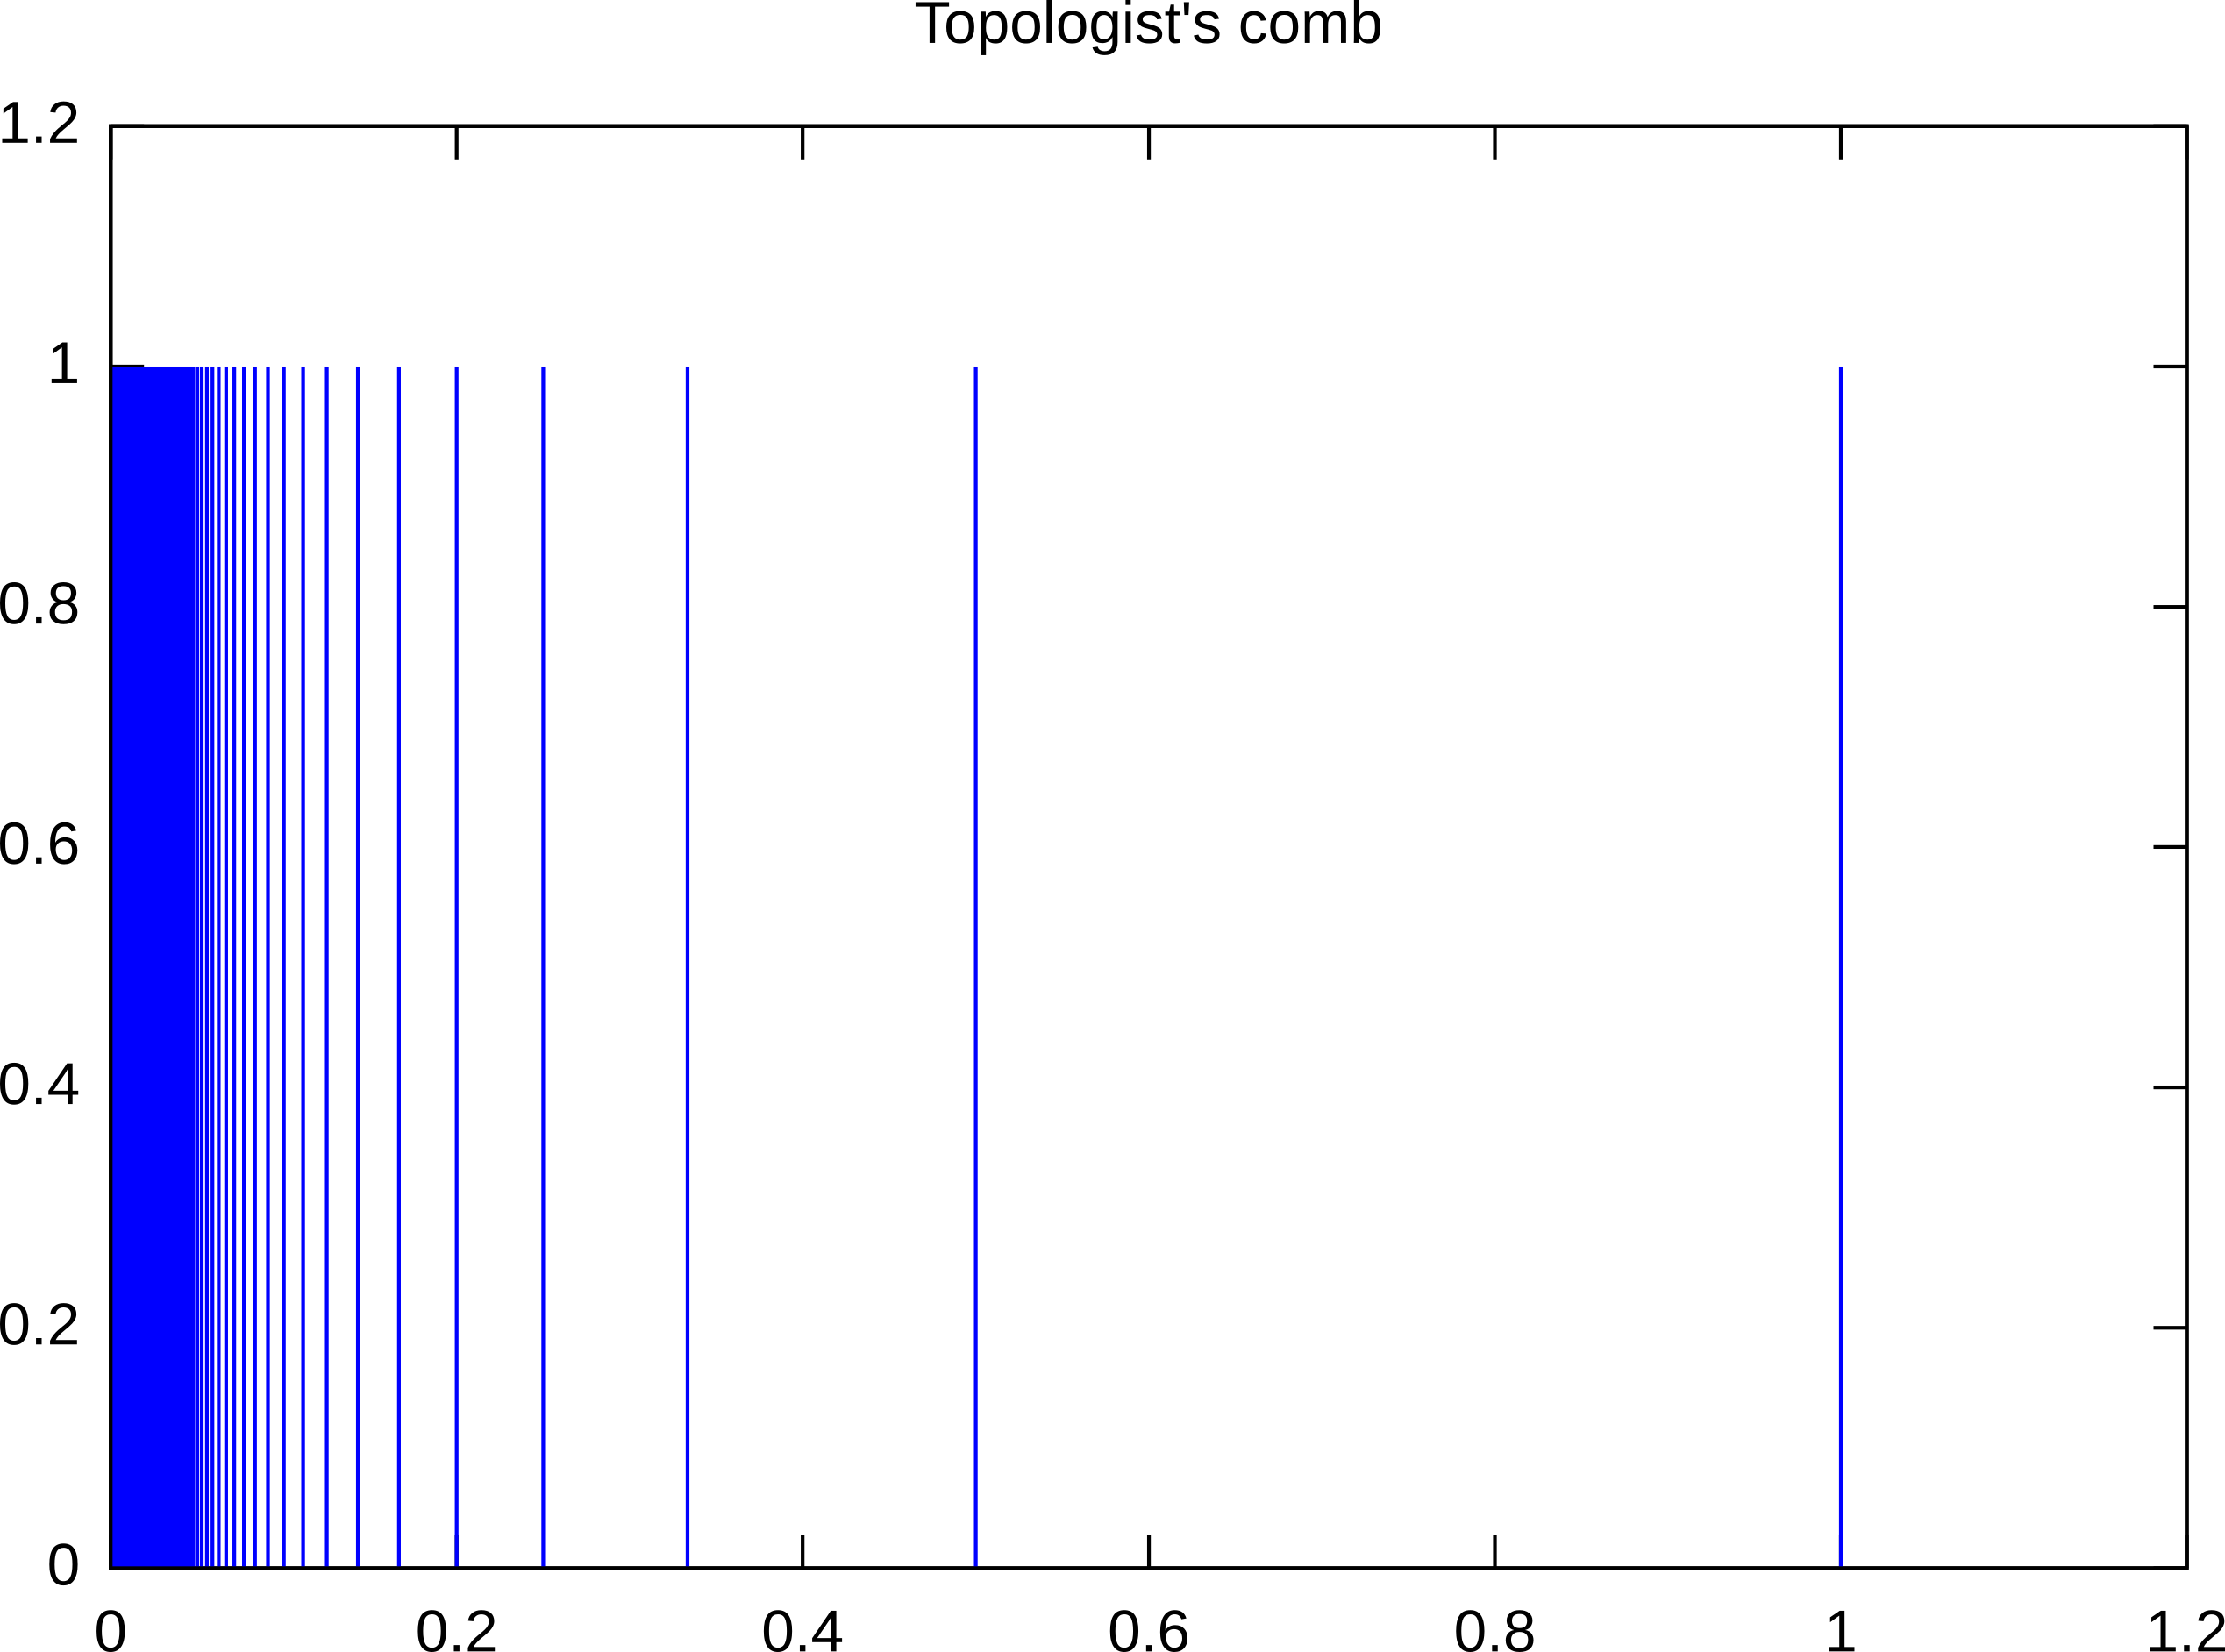
\includegraphics[width=0.5\linewidth]{images/topologia_generale/g160}
			\caption{Visualizzazione del pettine del topologo}
			\label{fig:comb_topology}
		\end{figure}
		
		
		Possiamo osservare che questo spazio è connesso. È ovvio che $D \setminus \left\{(0,1)\right\}$ è connesso per archi e quindi è connesso, pertanto se fosse sconnesso le componenti sarebbero $(0,1)$ e $D \setminus \{(0,1)\}$. Ma $\overline{D \setminus \{(0,1)\}} \cap \{(0,1)\} \neq \varnothing$ e quindi tutto $D$ è connesso. 
		
		D'altro canto $D$ non è connesso per archi. Consideriamo $f$ funzione continua che connette $(0,1)$ a $(0,0)$, con $f(0) = (0,1)$. Mostriamo che $f^{-1}(D)$ è sconnesso, da cui per assurdo si arriva che $\left[0,1\right]$ è sconnesso. Allora vediamo che $f^{-1}(\left\{0\right\})$ è chiuso per definizione (un punto è chiuso e la controimmagine di un chiuso è chiuso se la mappa è continua). Per cui dobbiamo far vedere che $f^{-1}(\left\{(0,1)\right\})$ è aperto. Prendiamo un intorno di $(0,1)$ che chiameremo $U \subset D$ dove tale da non intersecare l'asse delle ascisse e lo supponiamo tale che $f^{-1}(U)$ è connesso. Allora 
		poiché $U$ non interseca l'asse delle ascisse, dev'essere che $x \in V$ tale da essere della forma $x = (1/n, k)$ per qualche $n \in \N$ e $k \in \left(0,1\right]$. Osserviamo che ogni intorno contiene almeno un elemento di questa forma (perché sappiamo che si `accumulano' su $(0,1)$). Per cui sia $x \neq (0,1)$ allora $x = (1/n, k) \in U$ per cui possiamo trovare $1/n+1< r< 1/n$ per cui possiamo vedere che la controimmagine di $U$ si può separare nei seguenti insiemi disgiunti 
		\begin{equation*}
			f^{-1}(U) = f^{-1}((-\infty, r)\times \left[0,1\right]) \cup f^{-1}((r,+\infty)\times \left[0,1\right])
		\end{equation*}
		Pertanto possiamo dire che $U$ è sconnesso contro la nostra ipotesi di connessione. Risulta quindi che $f^{-1}((0,1))$ è aperto e chiuso, ma $\left[0,1\right]$ è ovviamente connesso da cui dev'essere che $\{(0,1)\}$ non è connesso per archi a $\{(0,0)\}$.
		
		\item Consideriamo la funzione reale 
		\begin{equation*}
			f(x) \coloneqq
			\begin{cases}
				0 & \text{se}\ x = 0 \\
				\sin \frac{1}{x} & \text{se}\ x \in \R^+
			\end{cases}
		\end{equation*}
		allora possiamo vedere in modo simile al pettine del topologo che l'immagine della funzione è connessa, ma il punto $(0,0)$ non è connesso per archi a nessun altro punto del grafo. Infatti se esistesse una funzione continua che collega le due parti del grafo avrebbe limite $\lim_{x\to 0} g(x) = \left[-1,1\right]$ e quindi non può essere continua in $0$.
	\end{enumerate} 
\end{remark}
